% This is "sig-alternate.tex" V2.0 May 2012
% This file should be compiled with V2.5 of "sig-alternate.cls" May 2012
%
% This example file demonstrates the use of the 'sig-alternate.cls'
% V2.5 LaTeX2e document class file. It is for those submitting
% articles to ACM Conference Proceedings WHO DO NOT WISH TO
% STRICTLY ADHERE TO THE SIGS (PUBS-BOARD-ENDORSED) STYLE.
% The 'sig-alternate.cls' file will produce a similar-looking,
% albeit, 'tighter' paper resulting in, invariably, fewer pages.
%
% ----------------------------------------------------------------------------------------------------------------
% This .tex file (and associated .cls V2.5) produces:
%       1) The Permission Statement
%       2) The Conference (location) Info information
%       3) The Copyright Line with ACM data
%       4) NO page numbers
%
% as against the acm_proc_article-sp.cls file which
% DOES NOT produce 1) thru' 3) above.
%
% Using 'sig-alternate.cls' you have control, however, from within
% the source .tex file, over both the CopyrightYear
% (defaulted to 200X) and the ACM Copyright Data
% (defaulted to X-XXXXX-XX-X/XX/XX).
% e.g.
% \CopyrightYear{2007} will cause 2007 to appear in the copyright line.
% \crdata{0-12345-67-8/90/12} will cause 0-12345-67-8/90/12 to appear in the copyright line.
%
% ---------------------------------------------------------------------------------------------------------------
% This .tex source is an example which *does* use
% the .bib file (from which the .bbl file % is produced).
% REMEMBER HOWEVER: After having produced the .bbl file,
% and prior to final submission, you *NEED* to 'insert'
% your .bbl file into your source .tex file so as to provide
% ONE 'self-contained' source file.
%
% ================= IF YOU HAVE QUESTIONS =======================
% Questions regarding the SIGS styles, SIGS policies and
% procedures, Conferences etc. should be sent to
% Adrienne Griscti (griscti@acm.org)
%
% Technical questions _only_ to
% Gerald Murray (murray@hq.acm.org)
% ===============================================================
%
% For tracking purposes - this is V2.0 - May 2012
%% LaTeX Preamble - Common packages

\documentclass{sig-alternate}
\usepackage{graphicx}
\begin{document}
%
% --- Author Metadata here ---
%\conferenceinfo{WOODSTOCK}{'97 El Paso, Texas USA}
%\CopyrightYear{2007} % Allows default copyright year (20XX) to be over-ridden - IF NEED BE.
%\crdata{0-12345-67-8/90/01}  % Allows default copyright data (0-89791-88-6/97/05) to be over-ridden - IF NEED BE.
% --- End of Author Metadata ---

\title{Text Mining Toolkit for Digital Humanities}



\numberofauthors{3} %  in this sample file, there are a *total*
% of EIGHT authors. SIX appear on the 'first-page' (for formatting
% reasons) and the remaining two appear in the \additionalauthors section.
%
\author{

\alignauthor
Olga Scrivner\\
    %   \affaddr{Institute for Clarity in Documentation}\\
      % \affaddr{1932 Wallamaloo Lane}\\
      % \affaddr{Wallamaloo, New Zealand}\\
       \email{olgas2@illinois.edu}
% 2nd. author
\alignauthor
Irina Trapido\\
    %   \affaddr{Institute for Clarity in Documentation}\\
    %   \affaddr{P.O. Box 1212}\\
    %   \affaddr{Dublin, Ohio 43017-6221}\\
       \email{trapido2@illinois.edu}
% 3rd. author
\alignauthor Jay Lee \\
      % \affaddr{The Th{\o}rv{\"a}ld Group}\\
      % \affaddr{1 Th{\o}rv{\"a}ld Circle}\\
    %   \affaddr{Hekla, Iceland}\\
       \email{lee9@illinois.edu}

}

\date{}


\maketitle
\begin{abstract}
Access to large digitized collections present a new opportunity to digital humanities researchers. At the same time, traditional methodology (e.g. close reading or keyword search) becomes very inefficient for literary data analysis. On the other hand, most available mining tools are built for different purposes and often require programming skills (even for software installation). Our project addresses these needs by optimizing a Shiny web application  that allows researchers to explore visually  and interactively their data collection. In addition, this application does not require any installation. While the core of this tool has been built, a lot of tuning and evaluation is needed, similar to META tool, in which  the user is able to select parameters. Finally, the current tool uses various topic modeling algorithms, each with a different parameter setting, thus providing their evaluation and guidance to a non-technical user is necessary.

\end{abstract}

% A category with the (minimum) three required fields
%\category{H.4}{Information Systems Applications}{Miscellaneous}
%A category including the fourth, optional field follows...
%\category{D.2.8}{Software Engineering}{Metrics}[complexity measures, performance measures]

%\terms{Theory}

\keywords{text mining, visualization, digital humanties}

\section{Introduction}


\section{Text Mining Techniques for Digital Humanities}


\section{Topic Modeling Tuning}
\section{Cluster Analysis}
\section{GUI optimization}
\section{Discussion and Conclusion}
Keeping Tables and figures as illustration how to use them in this format

\begin{table}
\centering
\caption{Frequency of Special Characters}
\begin{tabular}{|c|c|l|} \hline
Non-English or Math&Frequency&Comments\\ \hline
\O & 1 in 1,000& For Swedish names\\ \hline
$\pi$ & 1 in 5& Common in math\\ \hline
\$ & 4 in 5 & Used in business\\ \hline
$\Psi^2_1$ & 1 in 40,000& Unexplained usage\\
\hline\end{tabular}
\end{table}




\begin{table*}
\centering
\caption{Some Typical Commands}
\begin{tabular}{|c|c|l|} \hline
Command&A Number&Comments\\ \hline
\texttt{{\char'134}alignauthor} & 100& Author alignment\\ \hline
\texttt{{\char'134}numberofauthors}& 200& Author enumeration\\ \hline
\texttt{{\char'134}table}& 300 & For tables\\ \hline
\texttt{{\char'134}table*}& 400& For wider tables\\ \hline\end{tabular}
\end{table*}
% end the environment with {table*}, NOTE not {table}!

\begin{figure}
\centering
   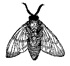
\includegraphics[width=1in]{fly.jpg}
\caption{A sample  (.jpg format).}
\end{figure}


\begin{figure*}
\centering
%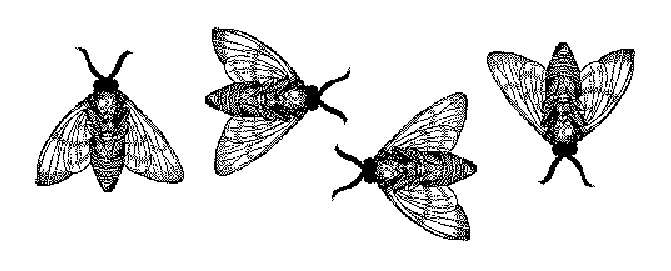
\epsfig{file=flies.eps}
   
\includegraphics[width=2in]{fly.pdf}
\caption{A sample figure
that needs to span two columns of text.}
\end{figure*}



\begin{figure}
\centering
%\psfig{file=rosette.ps, height=1in, width=1in,}
   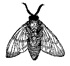
\includegraphics[width=1in]{fly.jpg}
\caption{A sample black and white graphic (.ps format) that has
been resized with the \texttt{psfig} command.}
\vskip -6pt
\end{figure}

\newtheorem{theorem}{Theorem}
\begin{theorem}
Let $f$ be continuous on $[a,b]$.  If $G$ is
an antiderivative for $f$ on $[a,b]$, then
\begin{displaymath}\int^b_af(t)dt = G(b) - G(a).\end{displaymath}
\end{theorem}


Citation \cite{salas:calculus} shown above,
use the \texttt{{\char'134}newtheorem} or the
\texttt{{\char'134}newdef} command,
respectively, to create it.




%\end{document}  % This is where a 'short' article might terminate

%ACKNOWLEDGMENTS are optional


%
% The following two commands are all you need in the
% initial runs of your .tex file to
% produce the bibliography for the citations in your paper.
\bibliographystyle{abbrv}
\bibliography{sigproc}  % sigproc.bib is the name of the Bibliography in this case
% You must have a proper ".bib" file
%  and remember to run:
% latex bibtex latex latex
% to resolve all references
%
% ACM needs 'a single self-contained file'!
%
%APPENDICES are optional
%\balancecolumns
%\appendix
%Appendix A
%\balancecolumns % GM June 2007
% That's all folks!
\end{document}
